%\documentclass[openany]{book}
\documentclass[12pt]{article}
\usepackage[utf8]{inputenc}
\usepackage{amssymb} %for fancy L
\usepackage{calrsfs} %for fancy L
\usepackage{cancel}
\usepackage{tabularx}
\usepackage[hyphens]{url}
\usepackage{booktabs}
\usepackage{graphicx}
\usepackage[titletoc,title]{appendix}
\usepackage{subfig}
\DeclareMathAlphabet{\pazocal}{OMS}{zplm}{m}{n} %for fancy L
\usepackage{epsfig, float,array,tabu,longtable,}
\usepackage{hyperref,wrapfig}
\usepackage{enumerate}
\usepackage{graphicx,psfrag}
\usepackage{enumitem}
\setlist{itemsep=0pt}
\usepackage{cite}
\usepackage{sectsty}
\usepackage{epstopdf}
\usepackage{amsmath,esint, setspace, fancyhdr, amsfonts, bookmark, blindtext}
\usepackage[normalem]{ulem}
\usepackage{tikz}
\usepackage{rotating}
\usepackage[americanvoltages,fulldiodes,siunitx]{circuitikz}
\usepackage{stackengine}
\usetikzlibrary{matrix}
\usepackage{multirow}
\usepackage{multicol}
\usetikzlibrary{shapes,backgrounds,patterns}
\usetikzlibrary{mindmap,trees,decorations.markings}
\usetikzlibrary{quotes,angles}
\usepackage{verbatim}
\renewcommand{\baselinestretch}{1}
\usepackage{natbib}
\setlength{\bibsep}{2.8pt}
\setlength{\textheight}{8in}
\setlength{\textwidth}{6.5in}
\setlength{\headheight}{0in}
\setlength{\headsep}{0.25in}
\usepackage{graphicx}
\setlength{\topmargin}{0in}
\setlength{\oddsidemargin}{0in}
\setlength{\evensidemargin}{0in}
\setlength{\parindent}{.3in}
\usepackage{listings}
\usepackage{color} %red, green, blue, yellow, cyan, magenta, black, white
\definecolor{mygreen}{RGB}{28,172,0} % color values Red, Green, Blue
\definecolor{mylilas}{RGB}{170,55,241}
\doublespacing

% remove double title from References section
\renewcommand\refname{}

\begin{document}


\begin{titlepage}

\newcommand{\HRule}{\rule{\linewidth}{0.5mm}} % Defines a new command for the horizontal lines, change thickness here

\center % Center everything on the page
 
%---------------------------------------------------------
%	HEADING SECTIONS
%---------------------------------------------------------

\textsc{\LARGE }\\[1.5cm] % Name of your university/college
\textsc{\Large Expression of Interest}\\[0.5cm] % Major heading such as course name
\textsc{\large }\\[0.5cm] % Minor heading such as course title

%---------------------------------------------------------
%	TITLE SECTION
%---------------------------------------------------------

\HRule \\[0.6cm]
{ \large \bfseries Coherent Elastic Neutrino-Nucleus Scattering  at the ESS}\\[0.4cm] % Title of your document
\HRule \\[1.0cm]
 
%---------------------------------------------------------
%	AUTHOR SECTION
%---------------------------------------------------------


%\begin{center} \large
%\medskip
%{\textsc{\textbf{Cole Mitchell} }}  \quad  {\textsc{\textbf{Matt %Policelli}}} 	\quad
%{\textsc{\textbf{Maurcio Segovia} }}  \quad 
%{\textsc{\textbf{Kyra Twohy} }}   % Your name, bold and small caps
%\end{center}
%\end{minipage}

%\begin{center} \Large
%{\textsc{\textbf{Group 7} }} 
%\end{center}

~
%\begin{minipage}{0.4\textwidth}
%\begin{flushright} \large
%\emph{Supervisor:} \\
%Dr. James \textsc{Smith} % Supervisor's Name
%\end{flushright}
%\end{minipage}\\[4cm]

% If you don't want a supervisor, uncomment the two lines below and remove the section above
%\Large \emph{Author:}\\
%John \textsc{Smith}\\[3cm] % Your name


\vspace{7mm}
%---------------------------------------------------------
%	DATE SECTION
%---------------------------------------------------------
\begin{center}
{\large \today}
\end{center}
 % Date, change the \today to a set date if you want to be precise
 \textsc{\small Document Number: }\\
 \textsc{\small Revision: 4}\\
  \textsc{\small State: Preliminary}\\
\vspace{21 mm}
%---------------------------------------------------------
%	LOGO SECTION
%---------------------------------------------------------
%\vfill
\newcommand*{\plogo}{
\includegraphics[width=0.35\textwidth]{ESS_logo.png}}

\plogo\\[1cm] % Include a department/university logo - this will require the graphicx package
 
%---------------------------------------------------------

\vfill % Fill the rest of the page with whitespace



\pagebreak
\newpage




\begin{table}[]
\begin{tabular}{lllll}
\cline{4-5}
 &                       & \multicolumn{1}{l|}{}                        & \multicolumn{1}{c|}{\textbf{Name}}                                                      & \multicolumn{1}{c|}{\textbf{Affiliation}}                                                  \\ \cline{3-5} 
 & \multicolumn{1}{l|}{} & \multicolumn{1}{l|}{\textbf{Main proposers}} & \multicolumn{1}{l|}{\begin{tabular}[c]{@{}l@{}}J.I. Collar\\ J.J. Gomez-Cadenas\\ F. Monrabal\\ C. Pe\~na-Garay\\ P. Privitera \end{tabular}}          & \multicolumn{1}{l|}{\begin{tabular}[c]{@{}l@{}}U. of Chicago\\ DIPC\\ DIPC\\ LSC \\ U. of Chicago \end{tabular}}              \\ \cline{3-5} 
 & \multicolumn{1}{l|}{} & \multicolumn{1}{l|}{\textbf{Co-proposers}}   & \multicolumn{1}{l|}{\begin{tabular}[c]{@{}l@{}}D. Baxter \\ P. Coloma\\ C.E. Dahl\\ I. Esteban \\ P. Ferrario \\ M. C. Gonzalez–Garcia\\ A.R.L. Kavner \\ C.M. Lewis \\ N. Lopez-March \\ J. Mu\~noz-Vidal\\ K. Ramanathan \\ J. Renner \end{tabular}} & \multicolumn{1}{l|}{\begin{tabular}[c]{@{}l@{}}U. of Chicago\\ IFIC\\ Northwestern U.\\ U. Barcelona\\ DIPC \\ Stony Brook U./U. Barcelona \\ U. of Chicago\\ U. of Chicago \\IFIC \\ DIPC \\ U. of Chicago \\ U. Santiago de Compostela \end{tabular}} \\ \cline{3-5} 
 &                       &                                              &                                                                                         &                                                                             
\end{tabular}
\end{table}
\pagebreak


\end{titlepage}


\clearpage
\newpage
\tableofcontents
\newpage     


% EXECUTIVE SUMMARY %%%%%%%%%%%%%%%%%%%%%%%%%%%%%%%%%%
\section{Executive Summary}

The European Spallation Source will soon provide the most intense neutron beams for
multi-disciplinary science. Conveniently, it will also generate the
largest pulsed neutrino production rate suitable for the detection and study of Coherent
Elastic Neutrino-Nucleus Scattering (CE$\nu$NS), a process recently
measured for the first time at ORNL's Spallation Neutron Source. CE$\nu$NS holds the potential for significant advances in sensitivity to numerous aspects of particle and nuclear phenomenology, providing a new, long-sought tool in the search for physics beyond the Standard Model.\\

We propose to use innovative nuclear-recoil detector technologies, optimized to profit
from the order-of-magnitude increase in neutrino production that is expected from 
the ESS when compared to all other existing or planned spallation sources. These low-cost, compact, unintrusive devices profit from previous R\&D aimed at other particle physics applications. They can be deployed coincident with the start of the ESS user program, without any significant impact or deviation from the ESS neutron mandate. The combination of a state-of-the-art performance from these advanced detectors, together with the uniqueness of the ESS as a high-yield pulsed neutrino source, will return high-statistics, precision CE$\nu$NS
measurements at the limit of the sensitivity to new physics reachable through this novel neutrino interaction mechanism. \\

Exploiting the exciting new development and opportunity that CE$\nu$NS represents, the program described here will significantly expand the physics reach of the ESS to a new area, that of neutrino physics, at the expense of just a minimal investment of resources. 

\newpage

% Scientific Opportunity %%%%%%%%%%%%%%%%%%%%%%%%%%%%%%%%%
\section{Science Case and Opportunity}

Neutrinos with energies below few tens of MeV  undergo a large enhancement to their cross-section for  elastic scattering off nuclei \cite{freedman,leo}. This mechanism is typically referred to as coherent elastic neutrino-nucleus scattering (CE$\nu$NS). During this neutral-current interaction, all nucleons participate coherently in the scattering process. The contribution from protons is markedly diminished by the numerical value of the weak mixing angle, resulting in a coupling effectively proportional to the square of the number of neutrons in the target nucleus \cite{leo}. This large enhancement to the scattering cross-section makes of CE$\nu$NS the  most probable mechanism for low-energy neutrino interaction, resulting in a substantial  detector miniaturization. Despite this marked advantage, the process remained undetected until 2017, more than four decades after its theoretical description. This counterintuitive delay resulted from the modest energy of the nuclear recoils induced -the single observable from this process-, and from the limited intensity of available neutrino sources in this energy range. First  evidence for CE$\nu$NS \cite{science,bjorn} was obtained using a 14.6 kg low-background sodium-doped cesium iodide detector \cite{ournim} exposed to the neutrino emissions from ORNL's Spallation Neutron Source (SNS), a precursor facility to the European Spallation Source (ESS). \\

 A number of tests for new physics are possible using CE$\nu$NS-sensitive neutrino detectors. For instance, a neutral-current detector responds almost identically to all known neutrino types \cite{diff}: observation of neutrino oscillations in such a device 
would provide unequivocal direct evidence for sterile neutrino(s) \cite{leo}. In addition to this, the differential cross section for this process is strongly dependent on the value of the neutrino magnetic moment \cite{dodd}. Numerous  studies have described the sensitivity of CE$\nu$NS to non-standard neutrino interactions with quarks \cite{Barranco:2005yy,new2}, to the effective neutrino charge radius \cite{Bernabeu:2002pd}, to neutron density distributions  \cite{patton,patton2,nst1}, and to accelerator-produced dark matter candidates \cite{tayloe2}. Precise measurements of the CE$\nu$NS cross section can provide a sensitive appraisal of the weak nuclear charge \cite{larry}, and constraints on new gauge bosons \cite{shoemaker}. A more extensive review of the rich particle phenomenology that can be investigated through CE$\nu$NS is available from  \cite{ESS}.\\


In a seminal paper \cite{leo}, Drukier and Stodolsky described the prospects for CE$\nu$NS detection from a variety of low-energy neutrino sources (solar, terrestrial, supernova, reactor, and spallation source). Of these, spallation sources were highlighted as the most convenient, due to higher recoil energies -easier to detect- and pulsed operation -leading to a more favorable signal-to-background ratio-. While the main use for these facilities is as intense neutron sources, their protons-on-target (POT) produce positive pions, which preferentially decay at rest (DAR), generating a monochromatic flash of 30 MeV prompt $\nu_{\mu}$. This is followed by delayed  $\nu_{e}$ and $\bar{\nu}_{\mu}$ emissions with a broad energy (Michel spectrum, up to few tens of MeV), over the $\sim$2.2 $\mu$s timescale characteristic of $\mu$ decay. Specifically, the instantaneous neutrino flux 20 m away from the ESS spallation target is expected to be $\sim 1.4\times10^{10}$ cm$^{-2}$ s$^{-1}$ \cite{ESS}.\\


The physics potential of CE$\nu$NS studies at the ESS has been examined in a recent publication \cite{ESS}. To avoid repetition, in this document we only summarize and condense the arguments presented there in much more detail. The ESS is on schedule to provide first protons on target during 2021, generating by 2023 an order of magnitude increase in neutrino production with respect to the SNS (Fig.\ \ref{fig:fig1}).  Compact, low-cost detectors (few kg to few tens of kg) operated at the ESS, have the opportunity to produce CE$\nu$NS measurements not limited in sensitivity by signal statistics (Fig.\ \ref{fig:fig2}), but instead only  by the irreducible O(10)\%  systematic error associated to uncertainties in detector response and neutrino flux.  Differences in beam timing profile between the SNS and ESS were included in the analysis in \cite{ESS}, concluding that the increase in neutrino production more than compensates for their impact on background reduction. The outcome is that the ESS will provide the very best sensitivity to neutrino properties and other areas of phenomenology that can be achieved via CE$\nu$NS, from any foreseeable future neutrino source (Fig.\ \ref{fig:fig2}, Table I). The large CE$\nu$NS signal throughput expected at the ESS allows to keep the detectors small (Fig.\ \ref{fig:fig3}), and therefore unintrusive to ESS neutron operations.\\

\begin{figure}[H]
\begin{center}
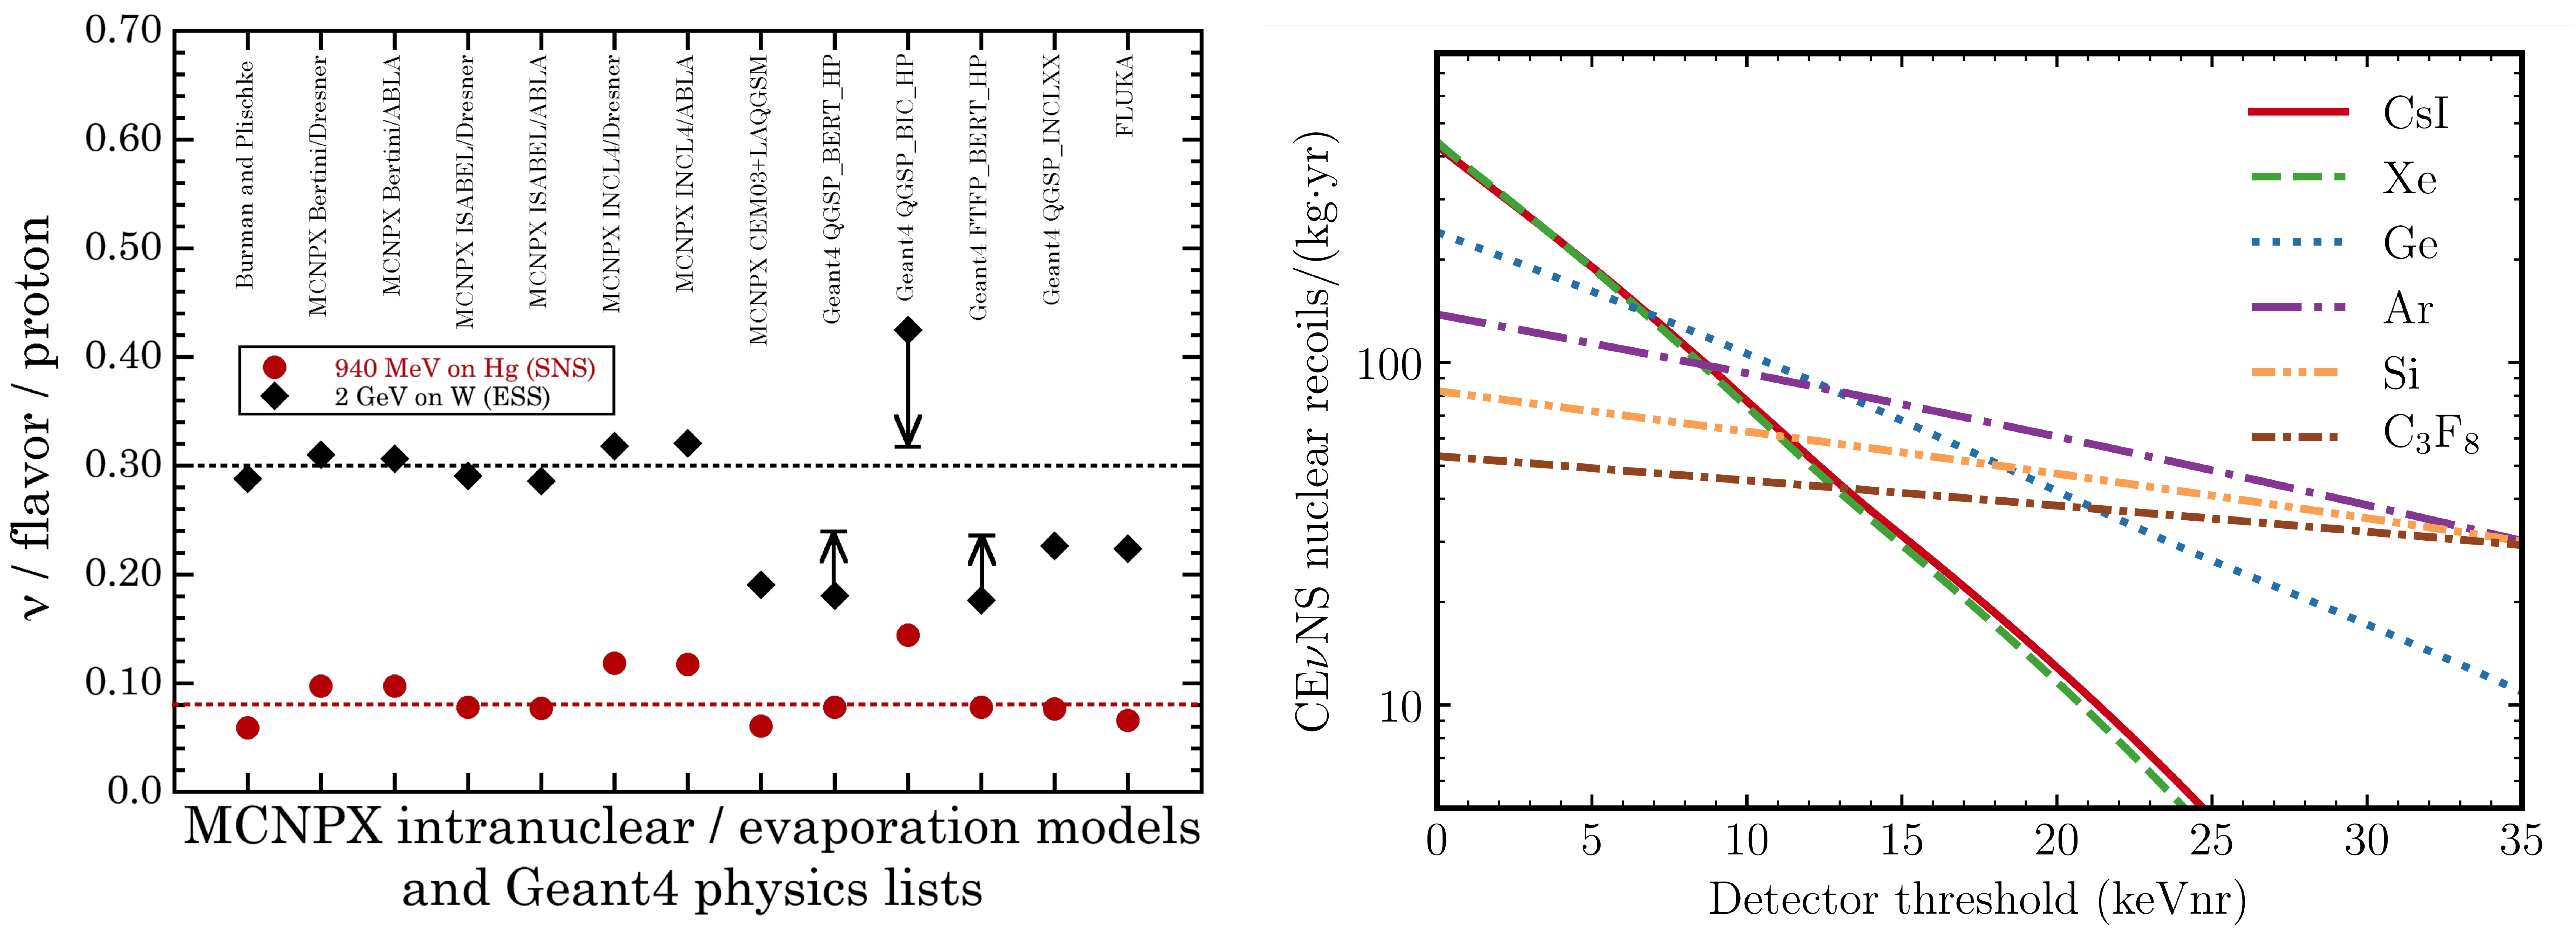
\includegraphics[width=5.1in]{fig1.eps}
\caption{\label{fig:fig1}\scriptsize {\it Left:} neutrino yields for the SNS mercury and
  ESS tungsten targets, obtained from different simulation packages. The first column shows predictions from a dedicated
  calculation \cite{burman,report}, validated against neutrino cross
  section measurements \cite{louis}. The combination of increased neutrino yield per proton and larger proton current on target of the ESS generates an increase in neutrino production rate by a factor 9.2 with respect to the SNS \cite{ESS}. {\it Right:} Expected integrated  CE$\nu$NS rate above nuclear recoil threshold, 20 m away from the ESS target, for detector materials examined in \cite{ESS}. All technologies considered for use at the ESS have state-of-the-art thresholds at or below 1 keV$_{nr}$. This maximizes sensitivity to new physics, which becomes most evident at the lowest recoil energies \cite{ESS}. }
\end{center}
\end{figure}

In the same publication we have described the opportunity to reinvest state-of-the-art nuclear recoil detectors already developed for other uses (e.g., DAMIC-M CCDs \cite{damic1,damic2,damic3,damic4} and scintillating bubble chambers \cite{eric} for WIMP detection, NEXT gaseous TPCs for double-beta decay \cite{next1,next2,next3}), for this purpose of CE$\nu$NS exploration (Fig.\ \ref{fig:fig3}). Our publication also describes novel technologies such as undoped cryogenic (80 K) CsI scintillators. This material, in combination with advanced light sensors and waveshifters, increases the CE$\nu$NS signal rate per detector mass by a factor of eight, with respect to the room-temperature CsI[Na] that was employed for the first CE$\nu$NS detection at the SNS. To provide some perspective, a compact 22 kg  CsI detector will register $\sim$8,000 CE$\nu$NS events per year at the ESS \cite{ESS}. This can be contrasted with the $\sim$3,000 events per year that a massive 750 kg liquid argon detector would achieve at the SNS \cite{tayloe}. Similarly-large signal rates are expected from other compact technologies proposed for use at the ESS \cite{ESS}. What is more, they are all able to reach nuclear recoil energies of $\lesssim$ 1 keV$_{nr}$. This maximizes their sensitivity to new physics, which appears preferentially at the lowest energies \cite{ESS}. This is again in contrast with the 20 keV$_{nr}$ threshold that can be expected from LAr scintillation \cite{tayloe,tayloe2}. While some of the detector technologies we have proposed excel in specific areas (e.g., DAMIC silicon CCDs for neutrino magnetic moment studies, Table I), their combination is synergistic, both for improving sensitivity, and for the investigation of possible anomalies (Fig.\ \ref{fig:fig2}, \cite{ESS}).   \\


\begin{figure}[H]
\begin{center}

\includegraphics[width=5.3in]{fig2.eps}
\caption{\label{fig:fig2}\scriptsize {\it Left:} Large CE$\nu$NS signal statistics expected from a 22.5 kg cryogenic CsI detector installed 20 m from the ESS target \cite{ESS}. Improvements in neutrino production and detector performance provide a $\sim\times100$ increase in CE$\nu$NS signal throughput with respect to the room-temperature CsI[Na] originally employed at the SNS \cite{ESS}. The ability to distinguish prompt $\nu_{\mu}$ from delayed $\nu_{e}$, $\bar{\nu}_{\mu}$ neutrino emissions using recoil energy information can be exploited towards a sensitive search for sterile neutrinos \cite{carlos}.  {\it Right:} increase in sensitivity to a parametrization of non-standard neutrino interactions with quarks, obtained by combining several target materials at the ESS (in this example different gases within a NEXT chamber), compared to the SNS. A similar advantage in all other areas of interest is expected (Table I, \cite{ESS}), a result of the order of magnitude increase in neutrino production at the ESS, and of technological advances in the nuclear recoil detectors being considered.}
\end{center}
\end{figure}

\begin{figure}[H]
\begin{center}
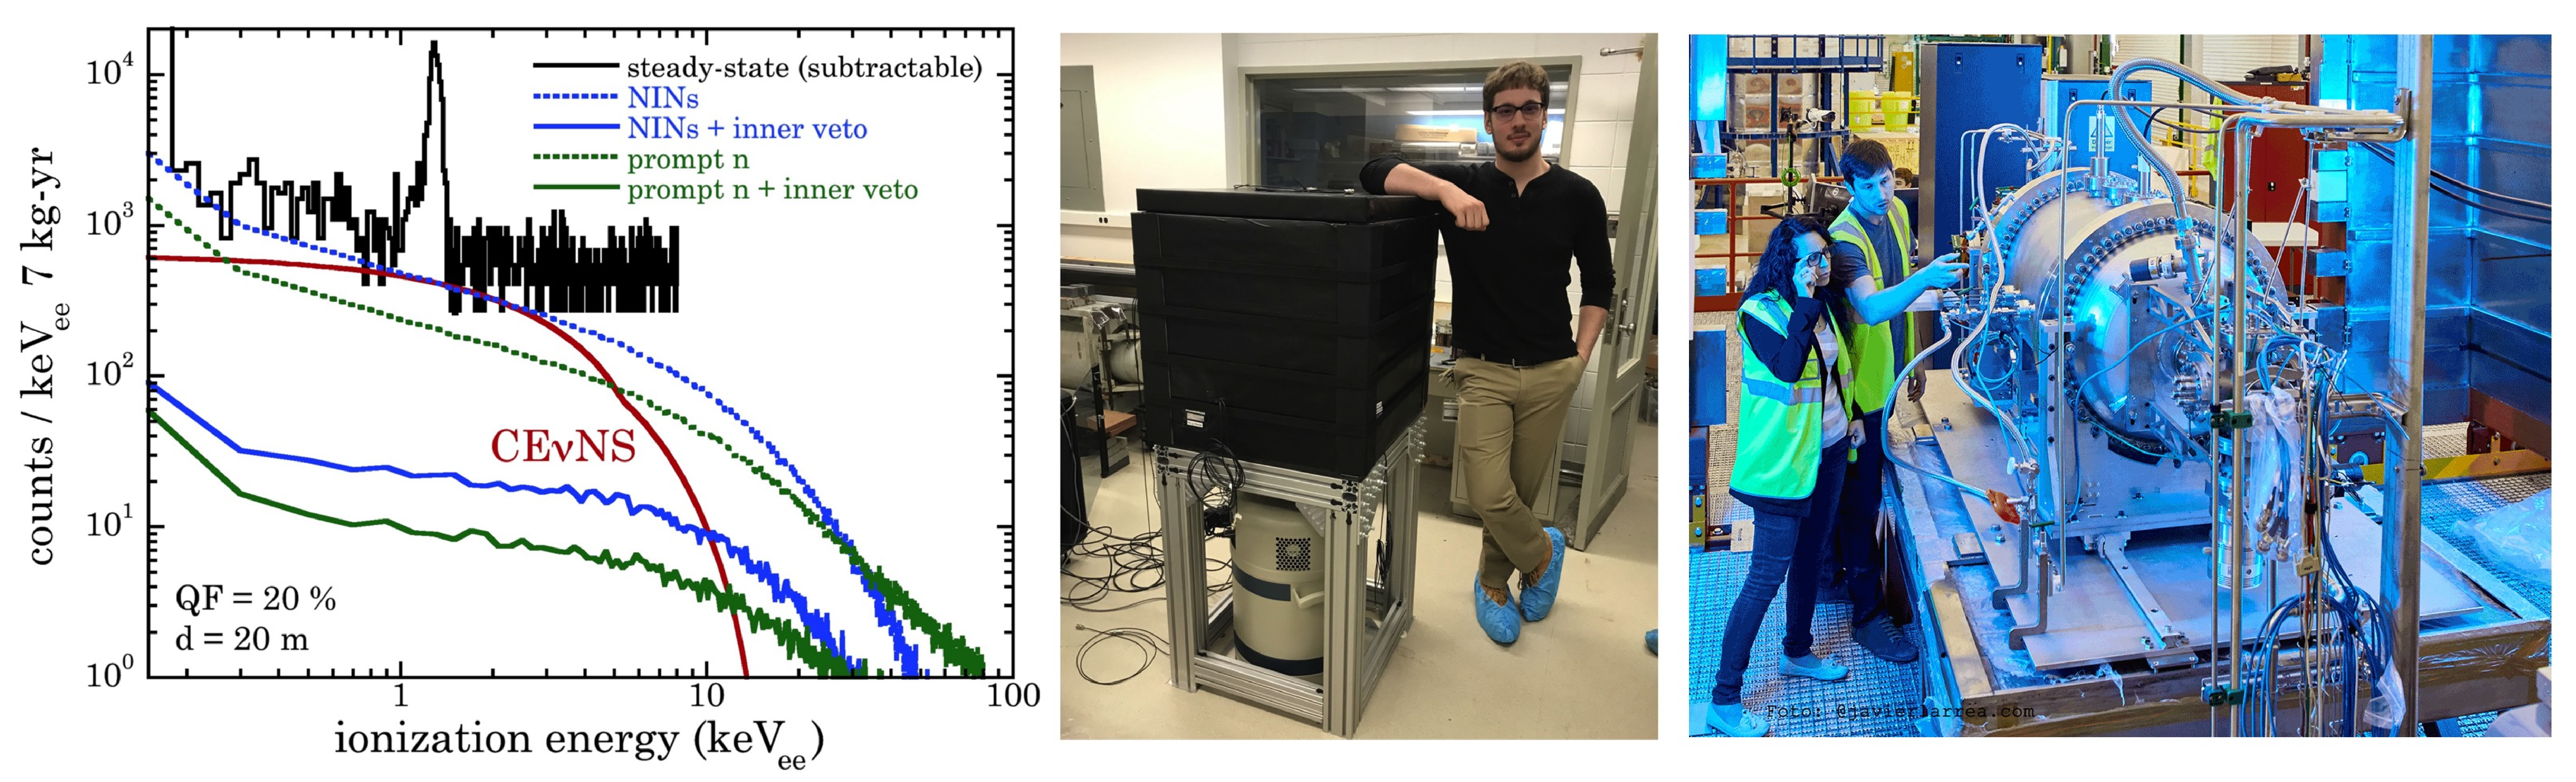
\includegraphics[width=6.5in]{fig3.eps}
\caption{\label{fig:fig3} \scriptsize {\it Left, center:} innovative, compact nuclear recoil detectors such as PPC germanium diodes \cite{ppc} are ready for an early ESS deployment. The plot shows a favorable comparison between simulated beam-related and measured steady-state (subtractable) backgrounds from the compact 3 kg PPC in the picture, against the expected CE$\nu$NS signal at the ESS. An overly conservative increase in beam-related backgrounds by a factor of ten with respect to our own measurements at the SNS  was adopted in the simulations \cite{ESS}. In an early stage of this project we envision a full characterization of ESS backgrounds via simulation and neutron measurements (Sec.\ 3). {\it Right:} The NEXT-White detector at the Canfranc underground laboratory (LSC). An envisioned chamber at the ESS will be similar in size, and will share many technical solutions already developed for this apparatus.}
\end{center}
\end{figure}


\begin{figure}[H]
\begin{center}
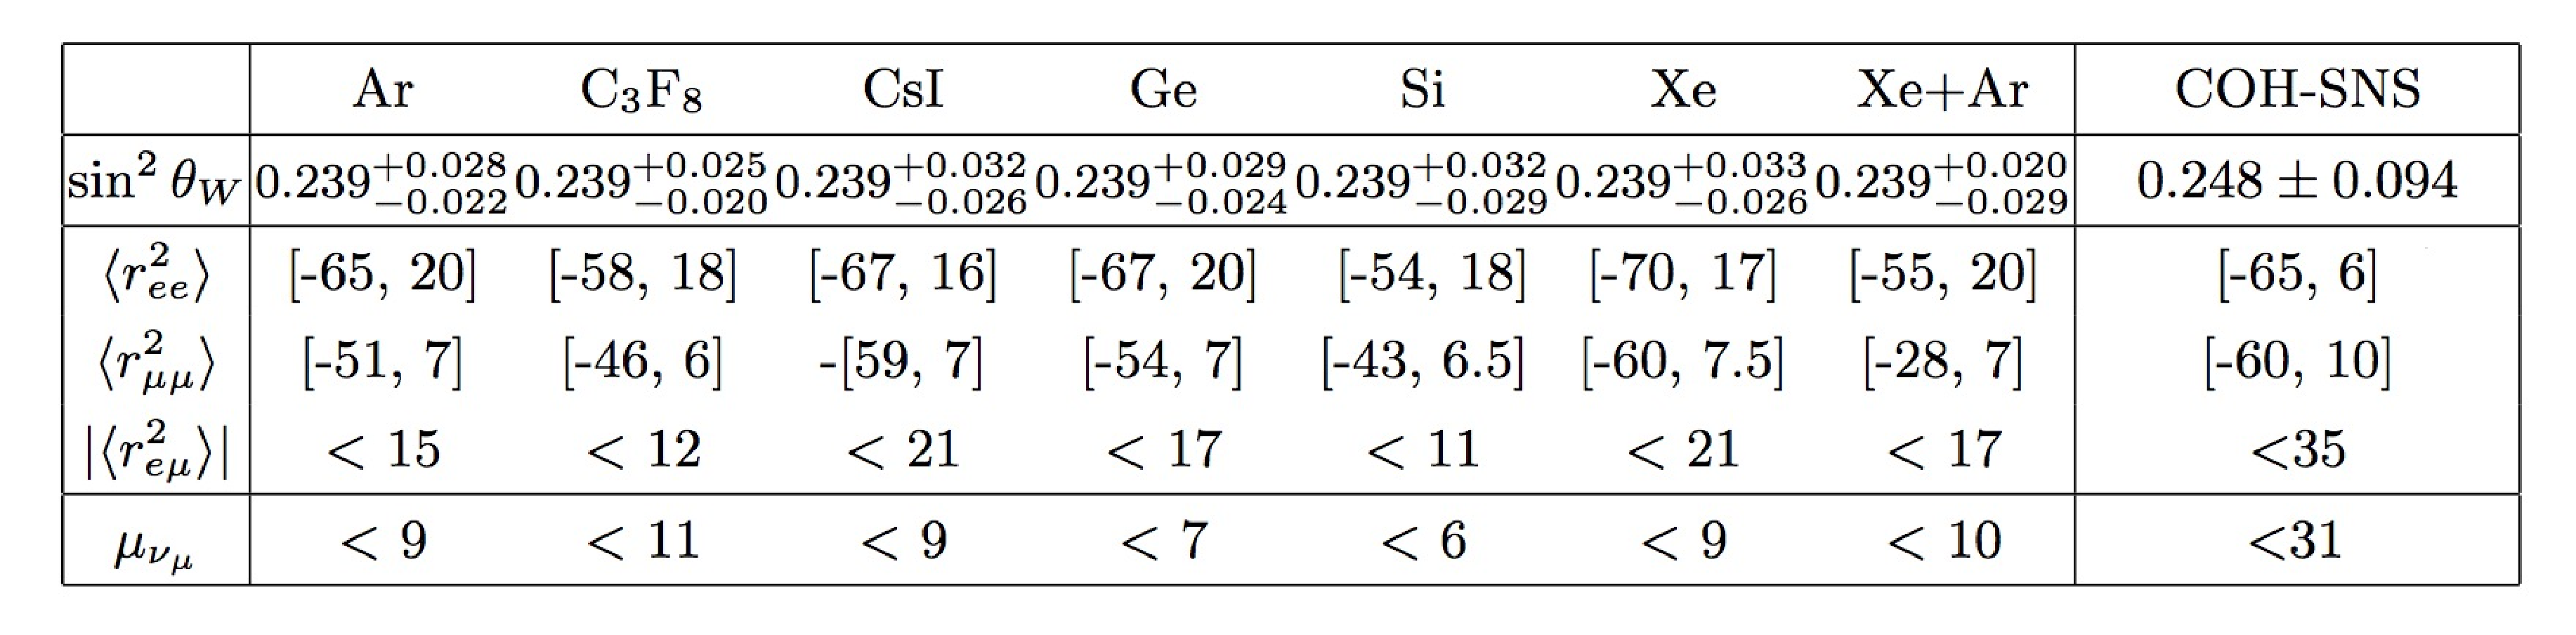
\includegraphics[width=6.5in]{table.eps}
\caption{\label{fig:figx} \scriptsize 
Table I: Allowed ranges at 90\% C.L. for the weak mixing
  angle (given as best fit $\pm 1.64 \sigma$), neutrino charge radii for three flavour
  projections  (in units of $10^{-32}$ cm$^2$, and after
  marginalizing over the other two flavour projections), and 
  the $\nu_\mu$ magnetic moment (90\% CL upper bound in units of
  $10^{-10} \mu_{\rm B}$) at the ESS, compared to the SNS (right column). The pion DAR neutrino production at the ESS is the largest of any present or planned spallation source, providing the best sensitivity to the many phenomenological applications of CE$\nu$NS \cite{ESS}. }
\end{center} 
\end{figure}





\newpage

% Timeline %%%%%%%%%%%%%%%%%%%%%%%%%%%%%%%%%%%%
\section{Timeline}

The time required to secure funding, design, and construct CE$\nu$NS detectors suitable for deployment at the ESS is an excellent match to the start of a neutron program in 2023. In some instances (e.g., ongoing DAMIC-M silicon CCD deployment at Modane), this is also well-aligned with  completion of detector use at other locations. The interim period can also be  utilized to perform neutron transport simulations aiming to validate the suitability of locations within the ESS facility,  already identified as potential  sites for unintrusive CE$\nu$NS experimentation (Fig.\ \ref{fig:fig4}). Neutron background measurements able to validate these simulations, similar to those already performed by us at the SNS (Fig.\ \ref{fig:fig5}, \cite{science,bjorn}), can commence as early as first ESS protons-on-target are produced. Over this early period, the possibility  of developing a conventional (i.e., not CE$\nu$NS-sensitive) $\sim$1-ton charged-current neutrino detector \cite{d2o} can also be studied. This additional activity would be beneficial for the whole program, as such a device  holds the potential to reduce a systematic uncertainty in the neutrino flux that can impact CE$\nu$NS sensitivity to new physics (Fig.\ \ref{fig:fig1}, \cite{ESS}). Calibrations of detector response to low-energy nuclear recoils, of crucial importance for the interpretation of results \cite{csiqf}, can also be performed during this preparatory period. \\

From the present perspective, a rough timeline can be sketched:


\begin{itemize}
\item {\bf 2020-2021:} funding applications, background simulations for site selection, detector design, detector response calibrations. Preparation of a Technical Design Report. 
\item {\bf 2022-2023:} neutron background measurements, deployment of first-ready technologies (e.g., germanium PPCs, Fig.\ \ref{fig:fig3}), detector construction and installation.  
\item {\bf 2024-2026:} CE$\nu$NS studies (sensitivity estimates \cite{ESS} assume 3-years of data-taking).
\item {\bf 2027-...:} In the event of detection of signatures of new physics, or if a large increase in sensitivity is foreseen by extrapolating a best-performing technology, concentration of resources on the design of a single larger detector can be contemplated at this point.  
\end{itemize}

\begin{figure}[H]
\begin{center}
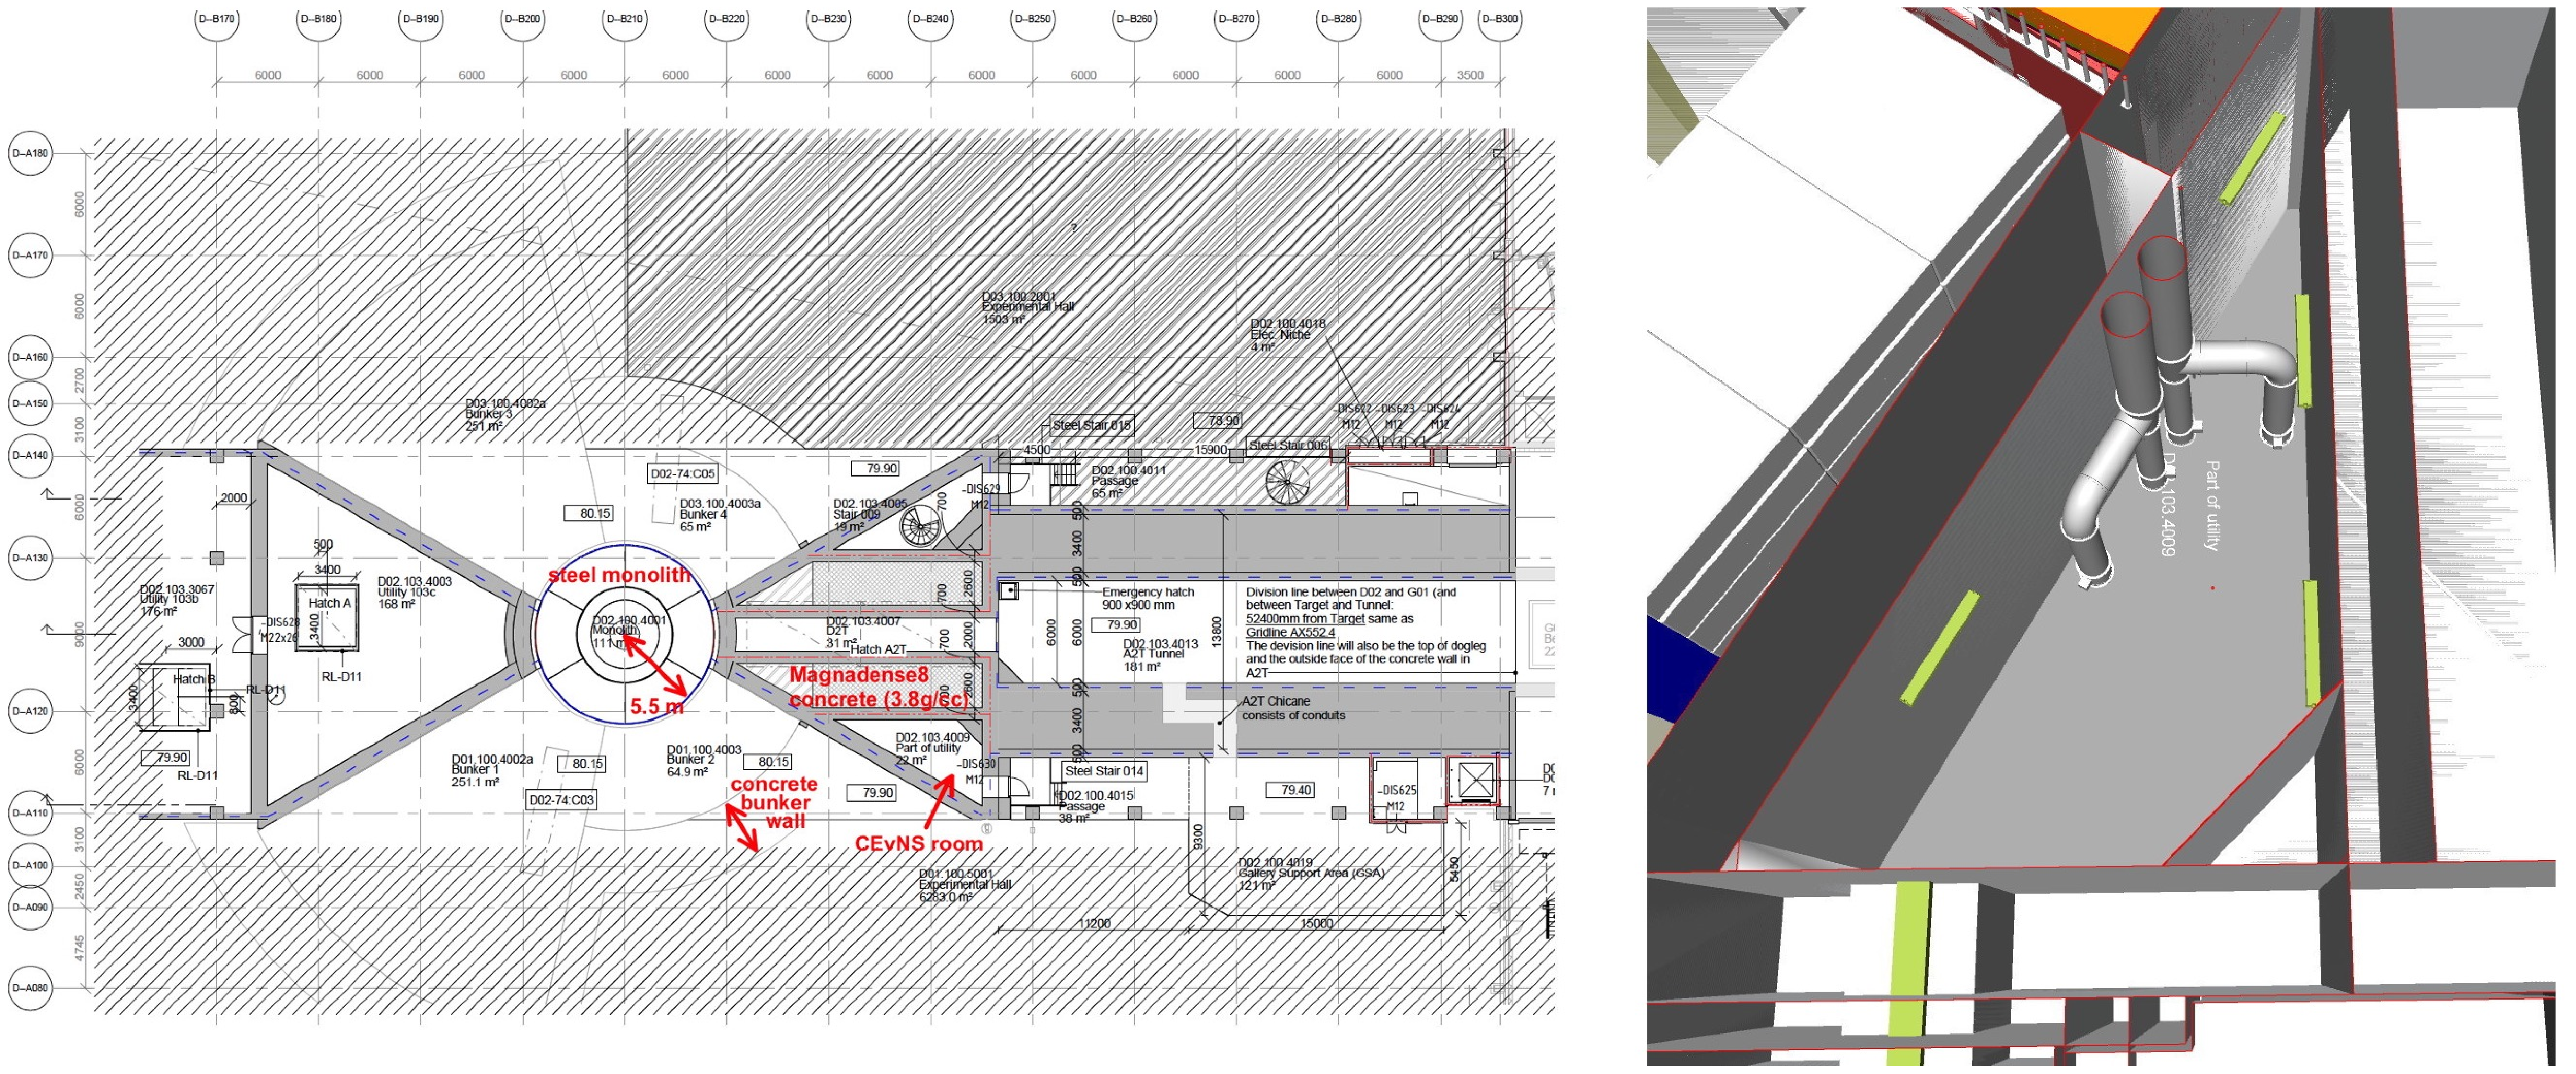
\includegraphics[width=5.7in]{fig4.eps}
\caption{\label{fig:fig4} \scriptsize ESS building layout indicating an unallocated room  identified as a possible site for CE$\nu$NS detectors, and NAVISWORKS 3-D visualization of this room. Two promising locations have already been identified, in collaboration with ESS personnel. The first is this room (15-23 m to target), featuring 5.5 meters of steel monolith and a minimum of 6 meters of magnetite-loaded  heavy  concrete  (3.8 g/cm$^{3}$) in  the  line-of-sight to target.  A second are underground galleries as close as 23 m to target, with compacted soil and concrete pylons separating them from the  monolith. Based on our previous experience in characterizing and simulating neutron backgrounds at the SNS, both locations hold great potential, to be confirmed via MCNPX simulations and neutron measurements. }
\end{center}
\end{figure}

\begin{figure}[H]
\begin{center}
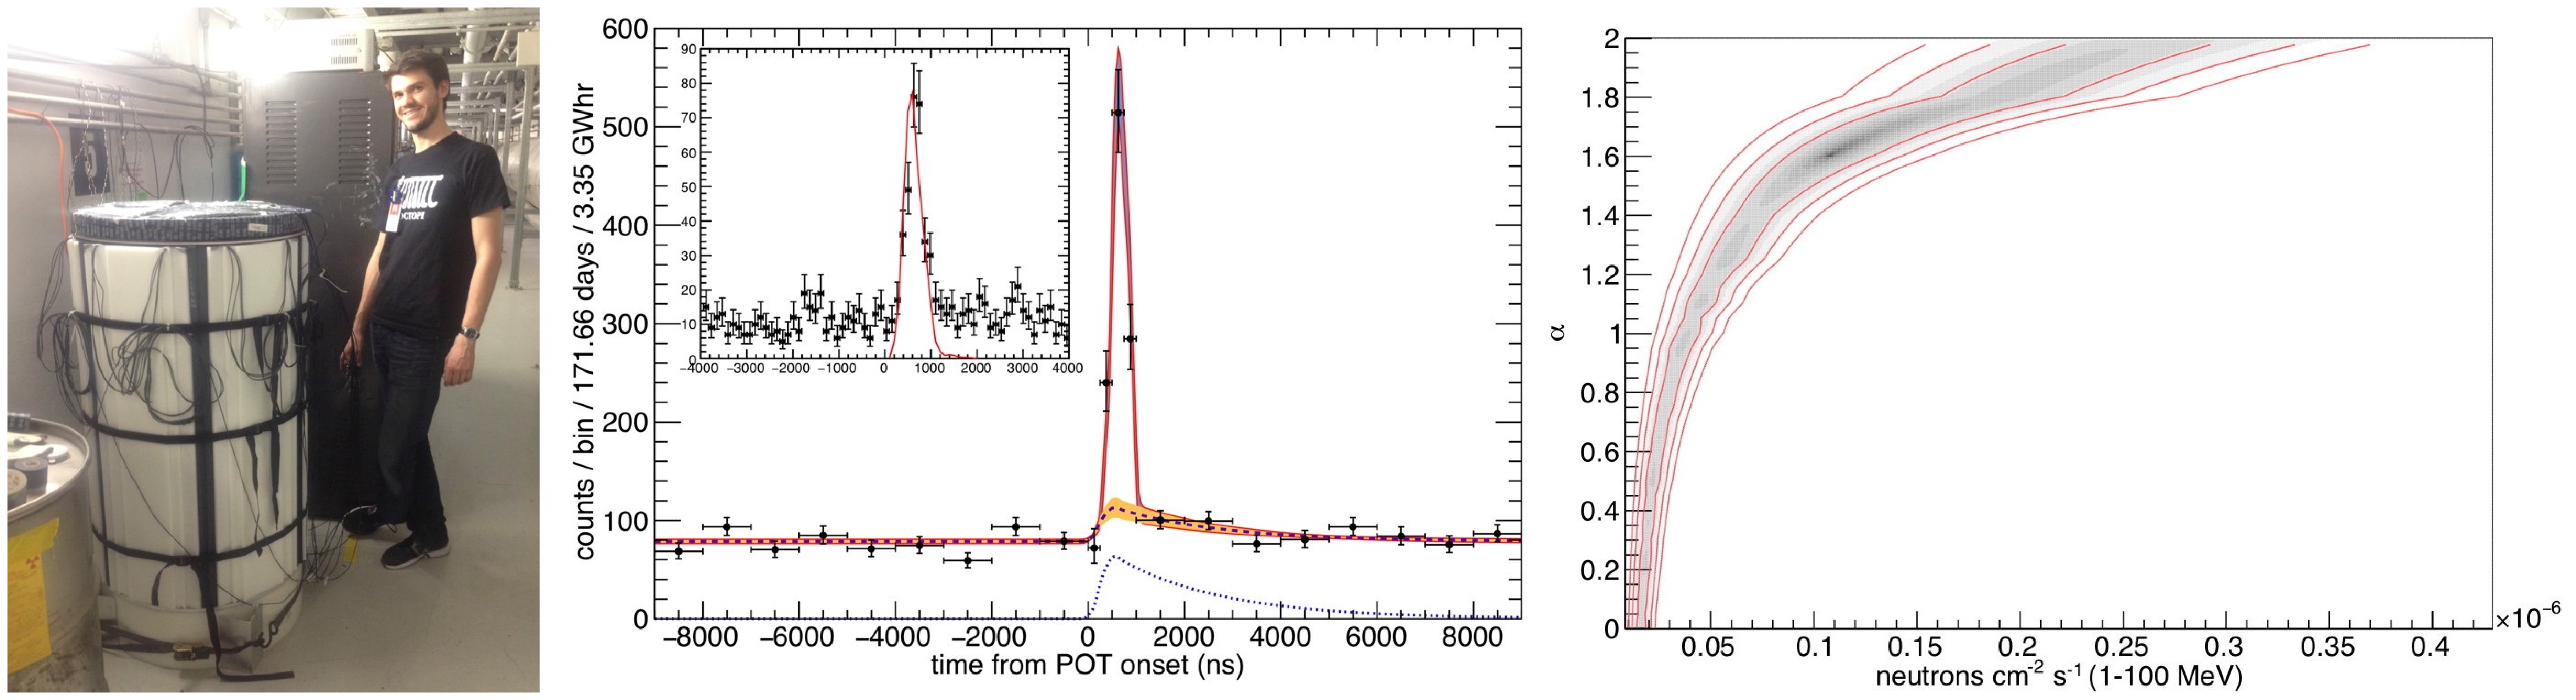
\includegraphics[width=6.2in]{fig5.eps}
\caption{\label{fig:fig5} \scriptsize {\it Left: }  former University of Chicago graduate student B. Scholz next to neutron detectors and dedicated shielding used for background studies at the SNS, prior to the first CE$\nu$NS measurement. This equipment exists and is available for similar studies at the ESS.  {\it Center:} (from \cite{science,bjorn}) beam-related background studies at the SNS. Both prompt neutron (central spike) and neutrino-induced neutron (NIN) backgrounds (yellow best fit) were measured or constrained using neutron-sensitive  scintillator cells. Similar studies are envisioned at the ESS once proton production has been initiated. {\it Right:} best-fit spectral hardness and flux for the small component of prompt neutrons detected at the CsI[Na] detector site during SNS background studies \cite{science,bjorn}. This is used to predict beam-associated backgrounds, allowing to select locations suitable for CE$\nu$NS experimentation. }
\end{center}
\end{figure}

\section{The $\nu$ESS collaboration}
The proponents of this physics program are in the process of organizing an international $\nu$ESS collaboration. Given the envisioned multi-detector nature of the experiment, the $\nu$ESS is conceived as a {\em Federation} which initially would include at least four major lines of experimental effort:
\begin{enumerate}
    \item {\bf Cryogenic scintillators}
     \item {\bf Low-background CCD arrays}
      \item {\bf High-pressure gaseous noble gas chambers}
     \item {\bf Neutrino and Neutron flux measurement detectors}
\end{enumerate}

Each line is led by a co-spokesperson (CSP) in charge of advancing his or her specific front. At the same time, the collaboration will organise a number of global working groups (GWG) which will include:

\begin{enumerate}
    \item {\bf Background characterisation of the site}
     \item {\bf Infrastructures}
      \item {\bf Monte Carlo simulation tools}
     \item {\bf Phenomenology and physics analysis}
\end{enumerate}

Lastly, the collaboration will perform R\&D towards a second generation of CE$\nu$NS neutrino experiments, which include scintillating  bubble  chambers and ultra-low threshold gaseous detectors, among other possibilities. \\

The scientific management of the collaboration will be the responsibility of the Federation Steering Committee (FSC), that will include the CSPs and the PIs of the GWGs. The FSC will be chaired by a coordination-spokesperson (XSP). The institutional management of the collaboration will be managed by the Federation Institutional Board (FIB), which will consist of the XSP, the CSPs (ex-officio members), one representative of the ESS and one representative of each of the institutions involved in the collaboration.\\

The following institutions are currently involved in the $\nu$ESS collaboration: Donostia  International  Physics  Center  (DIPC, San Sebasti\'an, Spain). Enrico Fermi Institute, University  of  Chicago (Chicago, IL, USA). Laboratorio Subterr\'aneo de Canfranc (LSC, Spain). Instituto  de  F\'isica  Corpuscular (IFIC, Valencia, Spain).  Departament  de  Fisica  Quantica  i  Astrofisica  and  Institut  de  Ciencies  del  Cosmos, Universitat  de  Barcelona  (Barcelona, Spain).  Basque  Foundation  for  Science (Ikerbasque,  Bilbao, Spain).  Instituci\'o  Catalana  de  Recerca  i  Estudis  Avancats  (ICREA, Barcelona, Spain).  Yang  Institute  for  Theoretical  Physics  (Stony  Brook  University, USA). Northwestern University (Chicago, IL, USA). Instituto 
Gallego  de  F\'isica  de  Altas  Energias,  Univ.  de  Santiago  de  Compostela, (Santiago, Spain). We expect that other institutions will join shortly. 

\newpage

% Costing \& ESS Support Expected %%%%%%%%%%%%%%%%%%%%%%%%%%%%%%%%%%%%
\section{Costing \& ESS Support Expected}

The development of a World-Class CE$\nu$NS program at the ESS requires, on one side, appropiate funding for the detectors, and on the other, a minimum of local support from the ESS.  Detector funding is to be sought during phase one, from EU and US sources, at no ESS cost. However, an early and firm commitment from the ESS to this activity would facilitate the obtention of this external funding. From the present perspective, and in view of the compact nature of the devices being considered, and of the maturity of the technologies involved, the funding necessary for detector construction should be  $<$20 MEUR. This rough upper limit includes the mentioned possibility of building a $\sim$1-ton charged-current detector for an accurate neutrino flux characterization.\\

Early access to the ESS, as soon as protons-on-target are generated, would be necessary  to perform the neutron background studies delineated in Sec.\ 3. In this respect of potential site identification,  a dynamic collaboration with ESS personnel is already taking place. Besides a suitable location(s) for the detectors, the minimal support envisioned from the ESS once CE$\nu$NS activities have started would include the allocation of some infrastructure, similar to what is provided to neutron instruments (local collaborators, power, POT trigger signals, supplies such as cryogens, data storage, safety supervision, office space, etc.).

\newpage

% Conclusion %%%%%%%%%%%%%%%%%%%%%%%%%%%%%%%%%%%%
\section{Conclusion}

CE$\nu$NS provides a new tool in the search for new physics beyond the Standard Model, one that spans both particle and nuclear realms. The technological maturity, small footprint, and low-cost of CE$\nu$NS-sensitive detectors, together with the unique intensity of the ESS as a pion DAR pulsed neutrino source, invite us to consider the development of a neutrino physics program at the ESS, with concentration on minimizing interference with neutron activities. However, we emphasize that the sensitivity of CE$\nu$NS investigations at the ESS depends critically on the neutrino production rate achieved, and therefore on reaching full design specifications of 5 MW power and 2 GeV proton energy, both in a timely fashion.\\

Given the opportunity, we intend to apply our accumulated experience in developing low-background nuclear recoil detectors, which includes the first CE$\nu$NS detection at the SNS, to create this new program of ESS activities. The net result will be a significant expansion of the ESS physics potential, in exchange for a modest investment of resources. 

\section{Acknowledgements}

We are indebted to M. Eshraqi, Z. Lazic, R. Linander, M. Lindros, V. Santoro, A. Takibayev, and L. Zanini at the ESS for their encouragement, and many useful consultations. We are also indebted to our colleagues...


% BIBLIOGRAPHY %%%%%%%%%%%%%%%%%%%%%%%%%%%%%%%%%%%%%%%
\newpage
\section{References}

\bibliographystyle{unsrt}
\bibliography{bibliography}
\fancyhead[R,OL]{bibliography}


\end{document}
